
\begin{frame}[noframenumbering,plain]
    \mytitle{Contributions}
    \bigskip
    \begin{columns}
	   \column{.57\textwidth}
      \begin{enumerate}
        \item Streaming Regular Expressions
        \item Gapped Consecutive Matching
        \begin{enumerate}
            \item Compressed Index
            \item Compressed Pattern Matching
        \end{enumerate}
        \item Run-reporting for unordered alphabets
        \item Approximate Longest Common Substring with approximately     mismatches
        \item Pattern Matching for the Dynamic Time Warping distance
        \item Compressing and Indexing Aligned Readsets
      \end{enumerate}
	   \column{.3\textwidth}
        \begin{framed}
            For each:
            \begin{itemize}
                \item Context
                \item Problem
                \item Results
                \item Use of sketches
            \end{itemize}
        \end{framed}
    \end{columns}
\end{frame}

\begin{frame}{A powerful matching model: regular expressions}
    \begin{columns}
        \column{.6\textwidth}
        \begin{mydefblock}{Regular expressions}
            either a character from $\Sigma$ or recursively defined from other regular expressions $R_1$ and $R_2$:
            \pause
            \begin{enumerate}
                \item $R_1 \cdot R_2$ (concatenation),
                \pause
                \item $R_1 | R_2$ (union),
                \pause
                \item $R_1^\ast$ (Kleene star).
            \end{enumerate}
            \pause
        \end{mydefblock}
        \column{.4\textwidth}
        \begin{center}
            \only<1|handout:0>{\textbf{Ex:} For $\Sigma=\{a,b\}$,\\ 
             $R_1=a$ only matches $a$,\\
             and $R_2=b$ only matches $b$.}
            \only<2|handout:0>{$R_1 \cdot R_2$ matches anything matching $R_1$ followed by anything matching $R_2$.\\
            \textbf{Ex:} with $R_1=a$ and $R_2=b$, $R_1 \cdot R_2$ matches $ab$.}
            \only<3|handout:0>{$R_1 | R_2$ matches anything matching $R_1$ or  $R_2$.\\
            \textbf{Ex:} with $R_1=a \cdot b = ab$ and $R_2=b$, $R_1 \cdot R_2$ matches $ab$ and $b$.}
            \only<4|handout:0>{$R_1^\ast$ matches any number of repetition of any string matching $R_1$.\\
            \textbf{Ex:} with $R_1=(b|ab)$ matches $\varepsilon$, $ab$, $b$, $bbabb$...}
            \only<5->{
                \textbf{Ex:} $b(b|ab)^\ast ab$\\
                \smallskip
                \cmark ~ $bbbbbabab$ \\
                \cmark ~ $bbbabbbbab$\\
                \xmark ~ $bbbaabbbab$\\
                \xmark ~ $baba$\\ 
                \xmark ~ $abab$\\
                }
        \end{center}
    \end{columns}    
    \pause
    \pause

    \bigskip
    \only<7->{Used in databases, \pause data mining, \pause secret detection,\pause computer networks, \pause protein search\pause ...\\}
    \pause
    \bigskip
    \only<12->{
        \beamermathcolor{myblue}
        Given a regular expression $R$ and a text $T$, two problems:\\
        \bblue{Membership:} check if $R$ matches $T$.\\
        \bblue{Pattern matching:} check if $R$ matches \textbf{some substring} of $T$. \pause \textcolor{myblue}{Reduces to membership!}
    }
\end{frame}

\begin{frame}{A frugal model of computation: streaming}
\begin{columns}
    \column{.4\textwidth}
    The algorithm first receives and preprocesses the expression.\\ Next, it keeps reading characters from a very very long text and:
    \column{.5\textwidth}
    \begin{center}
        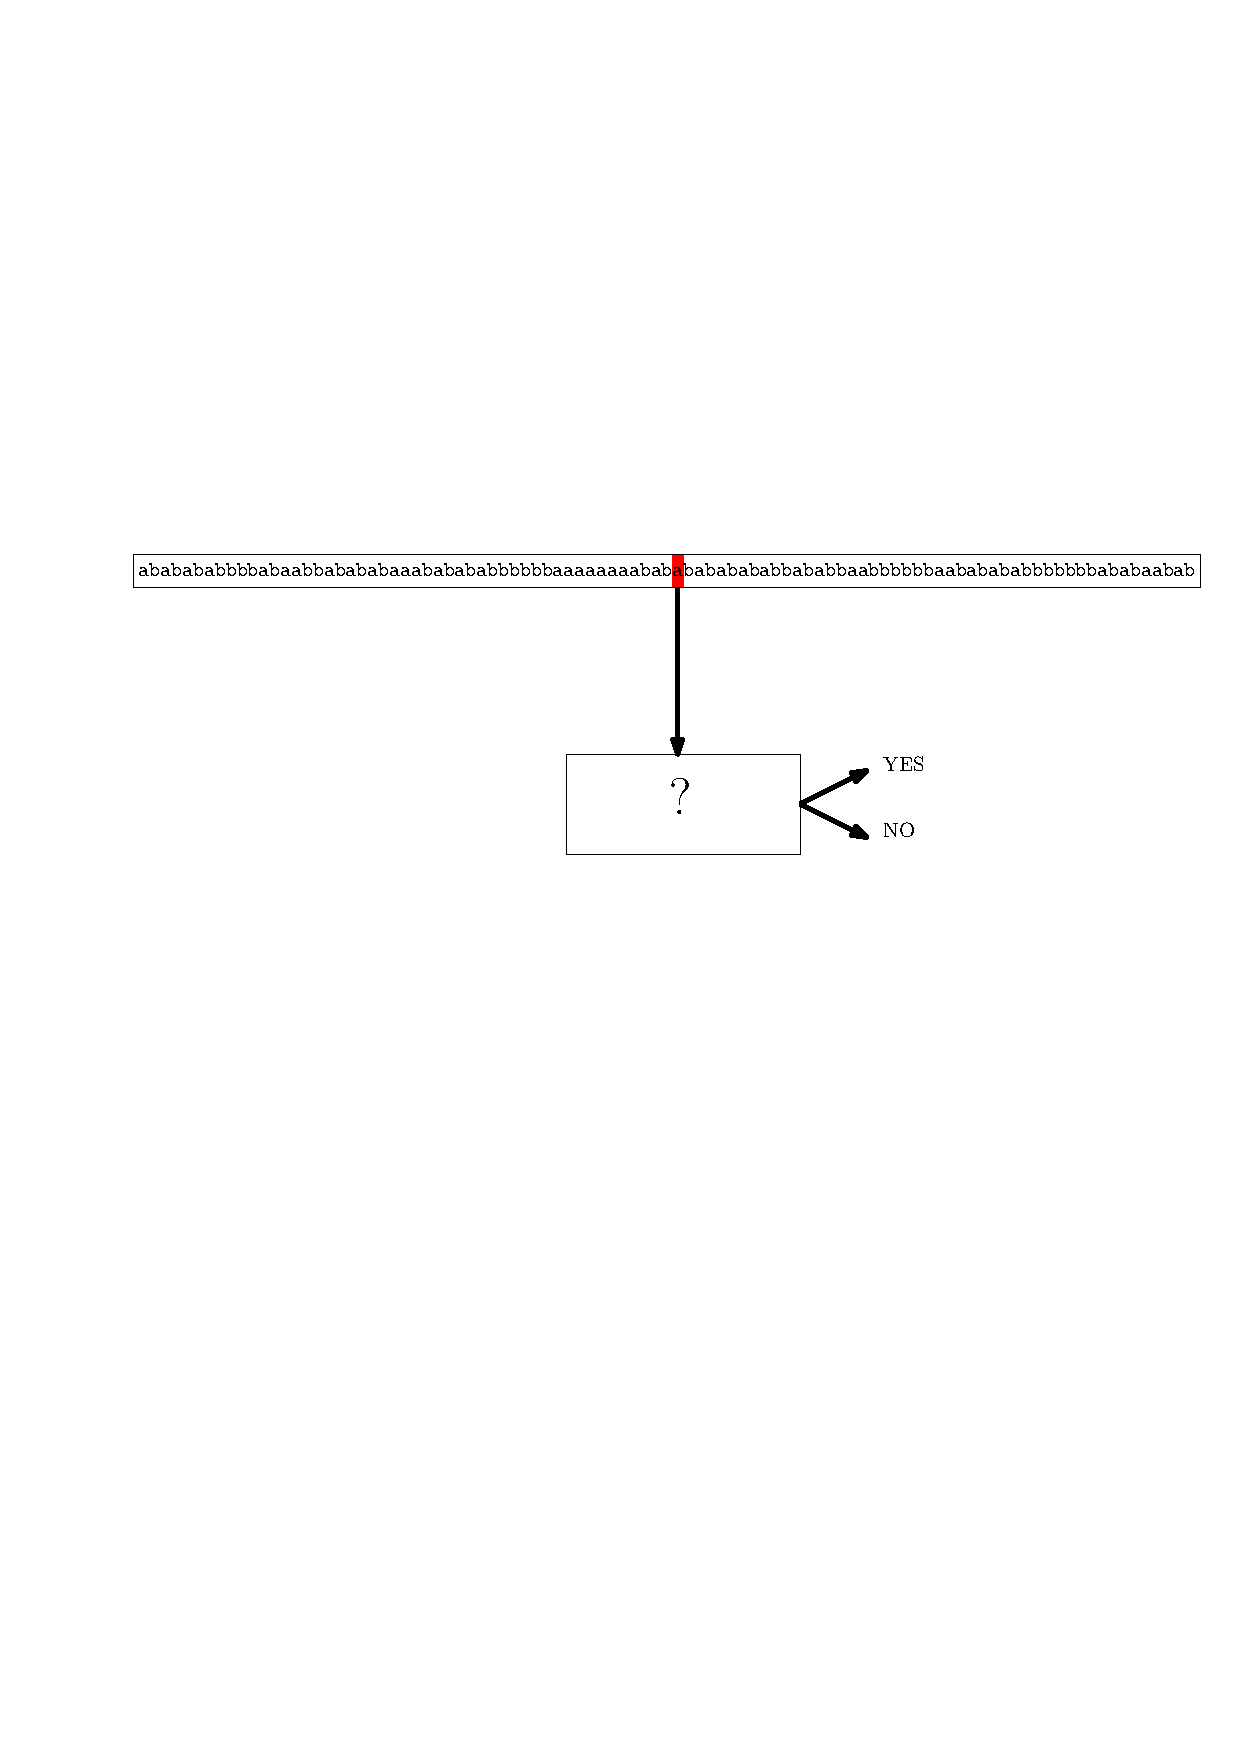
\includegraphics[width=\textwidth]{pictures/stream3}
    \end{center}
\end{columns}

\smallskip
\pause
\begin{enumerate}
\item No delay: After having seen the $i$-th character, immediately report whether the string so far matches the regular expression.
\pause
\item No going back: Not possible to read any of the earlier characters.
\pause
\item Every space counts: No access to the original expression (unless stored explicitly).
\end{enumerate}
\pause
\begin{mylemblock}{Classic pattern matching in streaming [Breslauer and Galil, TALG'14]}
    For a pattern of length $m$, it takes $\Oh(\log m)$ space and $\Oh(1)$ time per position.
\end{mylemblock}\pause
\begin{center}
    \small
    It relies on a variant of the Karp--Rabin fingerprints introduced by \ntheme{[Porat and Porat, FOCS'09]}.
\end{center}
\end{frame}

\begin{frame}{What can we do for regular expression membership in streaming ?}
    \begin{columns}
        \column{.35\textwidth}
        \ntheme{Classic:} Recursively build the \btheme{Thompson automata}, then check if $T$ is accepted.\\
        $\Oh(m)$ space and time/character.
        \column{.5\textwidth}
        \centering
        \begin{picture}(200,65)
            \put(0,0){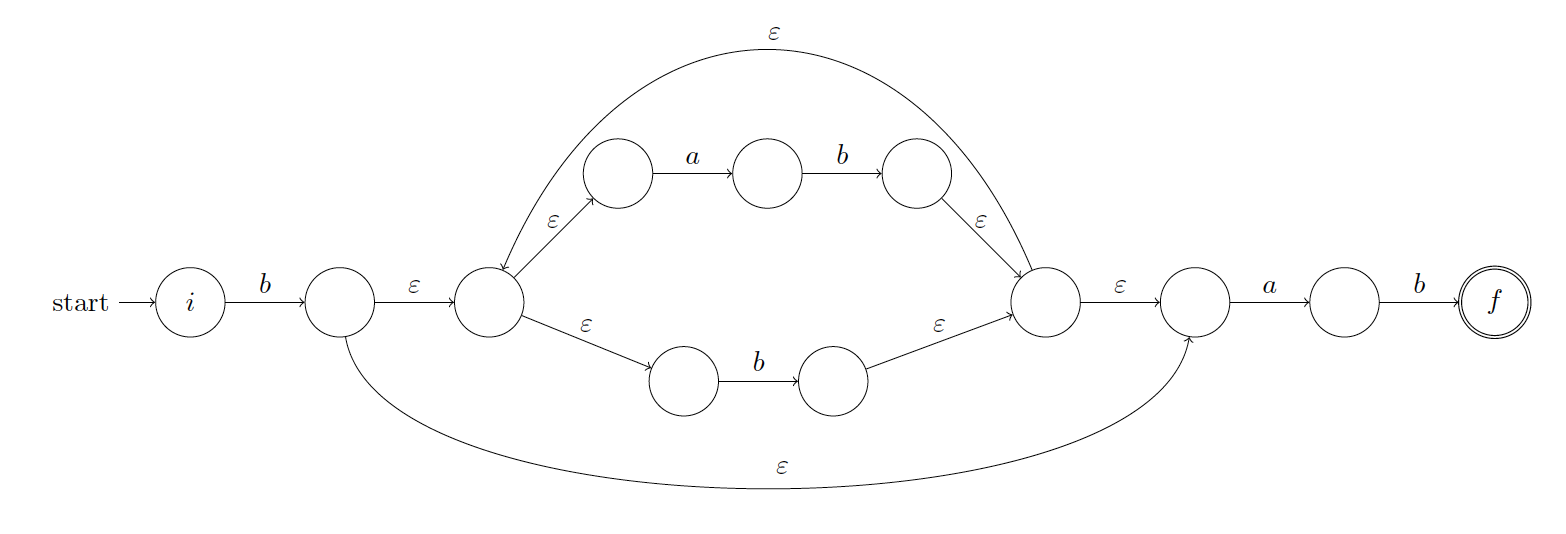
\includegraphics[width=\textwidth]{pictures/thomson1.png}}
            \put(150,50){\small $b(b|ab)^\ast ab$}
        \end{picture}
    \end{columns}
    \pause
    \begin{itemize}
        \item The best improvements on the time complexity \ntheme{only reduce by logarithmic factors}.\pause
        \item Fine-grained complexity showed that for \ntheme{``hard to match'' expressions we cannot do better}.\pause
        \item \ntheme{[Bille and Thorup, SODA'10]} Streaming time $\Oh(n\cdot (\frac{d\log w}{w}+\log d))$ and $\Oh(m)$ space, where $d$ is the number of occurrences of $|$ and $\ast$.\pause
        \item What about \btheme{space efficiency} ?\pause
    \end{itemize}
    


    \begin{myalertblock}{Dudek, Gawrychowski, Gourdel, Starikovskaya, SODA'22}
        For any regular expression $R$ with $d$ occurrences of $|$ and $\ast$, we can solve regular expression membership using $\Oh(d^{3}\polylog n)$ space and $\Oh(nd^{5}\polylog n)$ time per character.
    \end{myalertblock}\pause
    \textcolor{gray}{\small{\textbf{Techniques:} Streaming P.M., Compact Thompson Automata, Circuit Machinery...}}
\end{frame}

\begin{frame}{A simpler matching model: Gapped Consecutive Matching}
    % Regexp are hard to match
    Fine grained complexity prooved 
    % Many alternative considered 
    % A recent intrest in Gapped Consecutive matching
\end{frame}
